\section{Einleitung}
\label{sec:einleitung}
Das hier vorgestellte Individuelle Projekt befasst sich mit der Simulation des Laufzeitverhaltens von Komponentennetzwerken. Hierbei steht die Analyse eines Netzwerkes vor dessen Implementierung im Vordergrund. 
Das jetzt folgende praktisches Beispiel soll im Vergleich zur mathematisch exakten Berechnung den Sinn der Simulation verdeutlichen.

\subsection{Simulationsumgebung vs. mathematische Berechnung}
\label{sec:einleitung:simvsmath}
Zur Entwicklung eines Systems sollen eine Reihe von Komponenten eingesetzt werden, welche in Kombination die Dienste des Systems implementieren. Die Komponenten sind hierbei durch ihre Konnektoren, ihre Dienste, einen inneren Kontrollfluss und ihre Laufzeiteigenschaften gekennzeichnet. Weiterhin ist die Verkn�pfung der Komponenten untereinander durch den Entwickler des Systems vorgegeben.
\par
Ziel der Simulation soll die Auswertung der Dienste des Gesamtsystems sein. Hierbei spielt neben der Antwortzeit der einzelnen Dienste des Systems die Identifizierung von 'Flaschenh�lsen' innerhalb des Komponentennetzwerks eine Rolle.\\
Besteht das System ausschlie�lich aus linear zusammenh�ngenden Komponenten, deren Dienste der Reihe nach von einer ankommenden Anfrage durchlaufen werden, so gestaltet sich die Analyse des Systems recht einfach. Problemf�lle lassen sich anhand der Einzelzeiten identifizieren und die gesamte Antwortzeit kann durch Addition der Einzelzeiten relativ leicht ermittelt werden.\\
Beinhalteten die Komponenten innerhalb des Systems jedoch Verzweigungen, so m�ssen alle sich ergebenen Pfade einzeln berechnet und mit einer bestimmten Gewichtung gewertet werden.\\
Weiterhin ergibt es sich in Systemen h�ufig, das bestimmte Dienste einer Komponente von mehren Diensten des Gesamtsystems ben�tigt werden. Ein Beispiel hierf�r sind Dienste, die Daten aus einer Datenbank auslesen. Hierbei geht die Analyse des Systems �ber die Pfade hinaus. Es m�ssen nun die Antwortzeiten der Dienste der Komponenten dynamisch auf die Anzahl zu einem Zeitpunkt ankommender Anfragen angepasst werden.\\
�bersteigt die mathematisch exakte Analyse des Systems bereits hier die Grenzen des sinnvoll machbaren, so erscheint die exakte Berechnung bei der Verteilung der einzelnen Komponenten auf verschiedene Prozessoren als unm�glich.
\par
An dieser Stelle kann die Simulation ansetzen. Es werden nun nicht mehr die mathematisch exakten Gegebenheiten berechnet sondern anhand der Simulation eines Modells mit einer bestimmten Ungenauigkeit ermittelt. Weiterhin lassen sich bei der Simulation 'Flaschenh�lse' identifizieren, die bei der mathematischen Berechnung nur schwer zu ermitteln sind. Hierzu kann beispielsweise einfach das Zeitverhalten einer Anfrage Dienst f�r Dienst aufgezeichnet und hinterher ausgewertet werden. Bild \ref{pic:simul} zeigt schematisch eine solche Simulation.

\begin{figure}[ht]
\begin{center}
\fbox{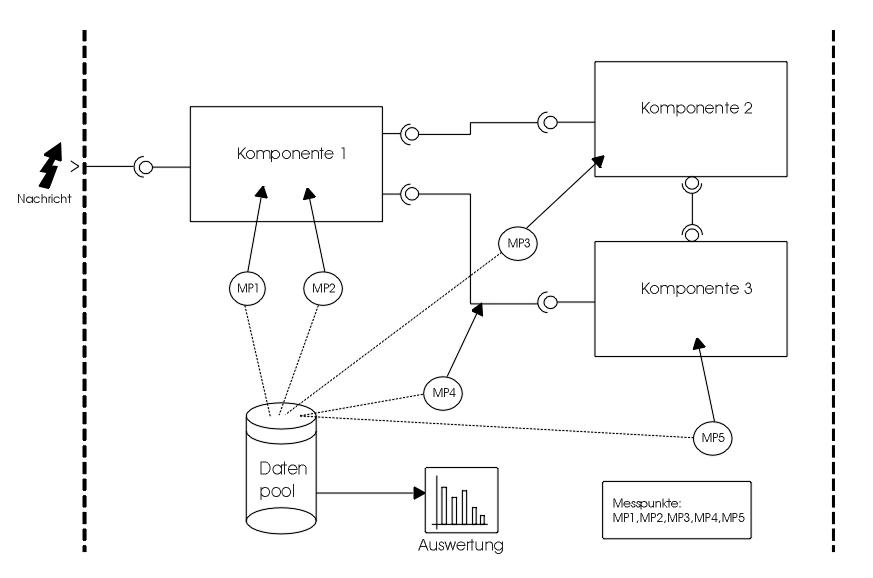
\includegraphics[width=13cm]{../res/simul.jpg}}
\caption{Schematische Darstellung der Simulation}
\label{pic:simul}
\end{center}
\end{figure}